\documentclass[12pt, a4paper]{article}
\usepackage[style=abnt]{biblatex}
\addbibresource{bibliografia.bib}
\usepackage[utf8]{inputenc} %Pacote para acentuação
\usepackage{csquotes}
\usepackage[portuguese,brazilian]{babel}
\usepackage[lmargin=3cm,tmargin=3cm,rmargin=2cm,bmargin=2cm]{geometry} %Formato que lembra a ABNT
\usepackage[T1]{fontenc} %Ajusta o texto que vem de outras fontes
\usepackage{amsmath,amsthm,amsfonts,amssymb,dsfont,mathtools,blindtext} %pacotes matemáticos
\usepackage{blindtext} %Texto aleatório
\usepackage{graphicx} %imagens
\usepackage{indentfirst}
\usepackage{booktabs, multirow} % for borders and merged ranges
\usepackage{soul}% for underlines
\usepackage[table]{xcolor} % for cell colors
\usepackage{changepage,threeparttable} % for wide tables
\usepackage{caption}
\usepackage{float}
\usepackage{multirow}
\usepackage{colortbl}
\usepackage{hhline}
\usepackage{array}
\usepackage{ragged2e}

\begin{document}

%% Capa
\begin{titlepage}
	\begin{center} %centralizar o texto abaixo
		{\begin{figure}[ht]
				\centering
				
\includegraphics[width=9cm]{imagens/logoUNESP.jpg}
			\end{figure}}
		{\bf \large FEIS – FACULDADE DE ENGENHARIA DE ILHA SOLTEIRA}\\[0.2cm] % o comando \\ "manda" o texto ir para próxima linha
		{\bf \large DEE – DEPARTAMENTO DE ENGENHARIA ELÉTRICA}\\[4cm]

        {\bf \large ENZO LUIZ FERNANDES}\\[4cm]

		{\bf \huge Plano de Trabalho de Graduação}\\[0.2cm] % o comando \bf deixa o texto entre chaves em negrito. O comando \huge deixa o texto enorme

		{\bf \Large Desenvolvimento e Análise de um Controlador Eletrônico de Velocidade para Motores de Corrente Contínua Sem Escovas}\\




	\end{center} %término do comando centralizar

	\vspace*{\fill} % Sempre na parte inferior da página
	\begin{center}
		{\large Ilha Solteira.}\\[0.2cm]

		{\large 2024}

	\end{center}
\end{titlepage}


%% Sumário
\newpage
\tableofcontents
\thispagestyle{empty}
\pagebreak


%-----------------------------------------------
\section{Introdução Teórica}

Os motores BLDC (\textit{Brushless Direct Current Motor}) representam um avanço significativo em relação aos motores CC tradicionais porque eliminam a necessidade de escovas mecânicas para a conversão de energia, resultando em maior rendimento energético, menos desgaste e maior vida útil \cite{hanselman2003brushless}. Esses avanços tecnológicos estão sendo impulsionados pela crescente demanda por sistemas de acionamento mais eficientes, confiáveis e de baixa manutenção em diversas aplicações industriais, comerciais e de consumo. A precisão e controlabilidade dos motores BLDC os tornam ideais para aplicações que exigem alta exatidão de movimento, velocidade e controle de torque, como robótica, automação industrial, veículos elétricos e eletrônicos de consumo.

\subsection{Motores CC Sem Escova}
O princípio de funcionamento dos motores BLDC é baseado em campos magnéticos gerados por ímãs permanentes e enrolamentos de  (Figura \ref{Configuração de um motor DC convencional (A) e motor BLDC (B).}). A comutação da corrente para gerar movimento ocorre eletronicamente, por meio de um controlador dedicado normalmente chamado de ESC (Eletronic Speed Controller), que pode usar ou não sensores durante o processo, eliminando assim a necessidade de escovas mecânicas utilizadas em motores DC tradicionais. Esta abordagem resulta em uma diminuição significativa do desgaste mecânico, aumentando a vida útil do motor e reduzindo a necessidade de manutenção.

\begin{figure}[h]
	\centering
	\caption{Configuração de um motor DC convencional (A) e motor BLDC (B).}
	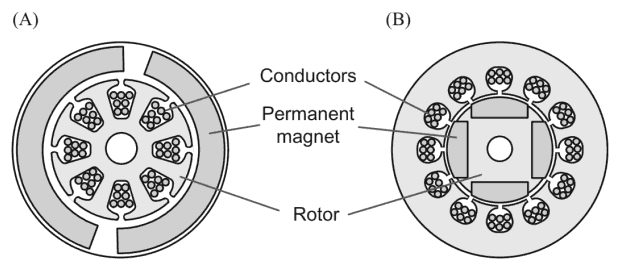
\includegraphics[width=8cm]{imagens/Comparativo.png}
	\caption*{Fonte:\cite{kim2017electric}.}
 \label{Configuração de um motor DC convencional (A) e motor BLDC (B).}
\end{figure}

Os motores BLDC são amplamente utilizados em uma variedade de aplicações, desde eletrônicos de consumo, como ventiladores e ferramentas elétricas, até aplicações industriais e automotivas. Sua capacidade de fornecer um controle preciso de velocidade e posição, juntamente com uma resposta rápida, faz deles a escolha ideal para sistemas que exigem rendimento energético e alta performance.

Apesar das muitas vantagens, os motores BLDC não estão isentos de algumas limitações. A complexidade eletrônica necessária para o controle preciso, o custo inicial potencialmente mais elevado comparado a motores elétricos escovados, a sensibilidade a ambientes de alta temperatura, pois podem gerar a desmagnetização dos imãs permanentes, a exigência de eletrônica de controle especializada, o potencial de ruído eletromagnético (EMI) e a complexidade de manutenção do sistema como um todo são fatores a serem considerados ao escolher essa tecnologia. Cada aplicação específica deve ponderar essas considerações em relação aos benefícios que os BLDC oferecem, como rendimento, durabilidade e controle superior.

\subsubsection{Princípios de Construção}

Motores BLDC são categorizados como síncronos, ou seja, o rotor gira na mesma frequência do campo magnético gerado pelo estator \cite{jahns1984torque}. Também não apresentam o fenômeno de escorregamento que é característico dos motores de indução. Os motores BLDC estão disponíveis em configurações de uma fase, duas fases e três fases, sendo  essa a mais amplamente utilizada, por serem equilibrados em relação a oscilação de torque e custo de construção \cite{hendershot1994design}.

\subsection{Controlador Eletrônico de Velocidade (ESC)}
Os controladores eletrônicos de velocidade, são dispositivos eletrônicos que controlam a velocidade e o torque de motores BLDC. São classificados pela sua corrente e tensão máxima de saída. São constituídos dos seguintes componentes básicos:

\begin{itemize}
\item Circuito de entrada: O circuito de entrada converte a tensão fornecida pela bateria em tensão que pode ser usada pelo circuito de controle utilizando PWM para gerar uma tensão média desejada que será fornecida ao motor. Também pode inverter a sequência de comutação das fases fazendo com que o sentido de rotação também seja invertido.
\item Circuito de controle: O circuito de controle é responsável por calcular a corrente que deve ser fornecida às bobinas do motor. Normalmente se utilizam de sinais com características de PWM como sinal de referência para definir a velocidade e sentido de rotação.
\item Circuito de saída: O circuito de saída fornece a corrente necessária às bobinas do motor.
\end{itemize}

Além desses componentes básicos, os ESCs para motor BLDC pode incluir os seguintes recursos, além dos já discutidos anteriormente:

\begin{itemize}
\item Filtro de ruído: O filtro de ruído é usado para reduzir o ruído elétrico que pode ser gerado pelo motor.
\item Proteção térmica: A proteção térmica é usada para proteger o motor de superaquecimento.
\item Proteção contra sobrecarga: O ESC pode desligar o motor se ele experimentar correntes superiores às nominais que representam riscos de deterioração das bobinas do motor.
\end{itemize}

\subsection{Princípios de Operação}

 O controlador do motor deve fornecer corrente e tensão adequadas às bobinas do estator do motor, a fim de controlar a velocidade e o torque do motor \cite{jahns1996pulsating}. O circuito básico que realiza esse papel é o de uma ponte inversora trifásica, onde o motor BLDC pode estar conectado em Estrela ou Delta. O controle do circuito de disparo dos transistores do inversor deve ser feito de forma que cada fase do estator seja percorrida por uma corrente com a forma de onda senoidal ou trapezoidal, voltadas respectivamente para alto rendimento e baixo custo. As formas de onda de cada uma das fases devem estar defasadas entre si, permitindo que o motor gire de forma contínua.

\subsubsection{Comutação de Seis Passos}

A comutação de seis passos demanda um sincronismo de disparo dos transistores, de modo que sempre dois deles estejam fechados, formando um circuito tal que a cada $60 ^\circ$ elétricos o par de fases percorridas pela corrente se alterne (Figura \ref{Sequência de acionamento para um BLDC trifásico}). Cada transistor permanece em condução durante $120 ^\circ$ elétricos. Vale ressaltar que os eventos de condução e bloqueio, denominados comutações dos transistores, geram variações na corrente e isso é responsável pelas oscilações no torque do motor \cite{kim2017electric}. 

\begin{figure}[p]
	\centering
	\caption{Sequência de acionamento para um BLDC trifásico.}
	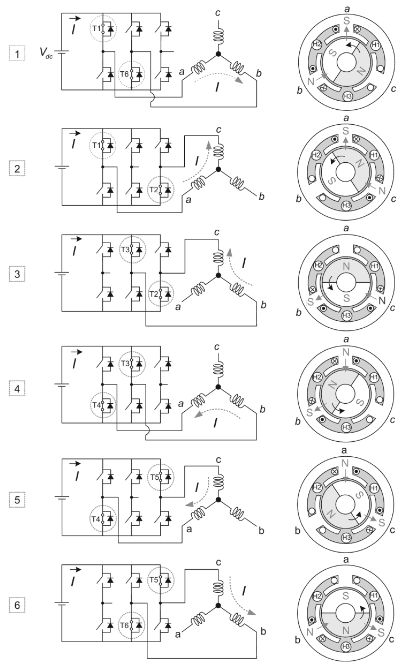
\includegraphics[width=10cm]{imagens/acionamento.png}
	\caption*{Fonte:\cite{kim2017electric}.}
 \label{Sequência de acionamento para um BLDC trifásico}
\end{figure}

Esse é o algoritmo de acionamento dos transistores mais amplamente utilizado para controlar motores BLDC e é também chamada de Controle Trapezoidal. Para se saber quando e quais deles acionar, existem duas opções, saber a posição que o rotor se encontra de forma a acionar o conjunto de transistores seguinte. Para esse tipo de controle se dá o nome de Controle de Malha Fechada. Também é possível acionar os indutores a partir de uma sequência fixa determinada pelo circuito, o que faz com que o rotor comece a girar em algum momento da sequência e siga girando a partir da sequência determinada. Esse tipo de controle é mais simples e de menor custo, porém não tão preciso, recebendo o nome de Controle de Malha Aberta.

 Para a realização do Controle de Malha Fechada é possível usar um sensor de efeito Hall capaz de identificar o campo magnético resultante da interação do campo eletromagnético das bobinas e do campo magnético dos imãs permanentes do rotor, indicando a seção que o campo eletromagnético resultante encontra-se, ou seja, sua posição angular. Partindo dessa referência, se pode saber quais transistores devem ser acionadas para que o rotor continue a girar. A utilização de sensor Hall também propicia a determinação da velocidade angular do motor. Esse método é mais complexo e de maior custo, porém garante uma maior confiabilidade em relação a velocidade.

Quando a aplicação necessita que o motor possua apenas uma velocidade, a fonte de alimentação de tensão fixa é suficiente, mas para casos onde é necessário varia a velocidade do motor precisa-se de uma ponte trifásica com controle PWM, um ESC por exemplo, entretanto essa técnica demanda a utilização de controladores que comparem a velocidade desejada da medida no rotor.

\newpage

\subsubsection{Modulação por Largura de Pulso}

Fontes de tensão fixa, como baterias, são as mais acessíveis do mercado. A partir delas, é possível gerar uma tensão média de alimentação variável utilizando uma técnica conhecida como PWM (Modulação por Largura de Pulso), permitindo o controle de velocidade de um BLDC. Para isso, utiliza-se um circuito simples capaz de transformar a tensão contínua em uma onda quadrada de frequência fixa e amplitude igual à tensão da fonte de alimentação. A própria ponte trifásica pode ajustar a largura dos pulsos, fazendo com que a tensão média entregue à ponte inversora seja proporcional à velocidade desejada (Figura \ref{Modulação por largura de pulso utilizando uma fonte de 100V}).

\begin{figure}[h]
	\centering
	\caption{Modulação por largura de pulso utilizando uma fonte de $100V$.}
	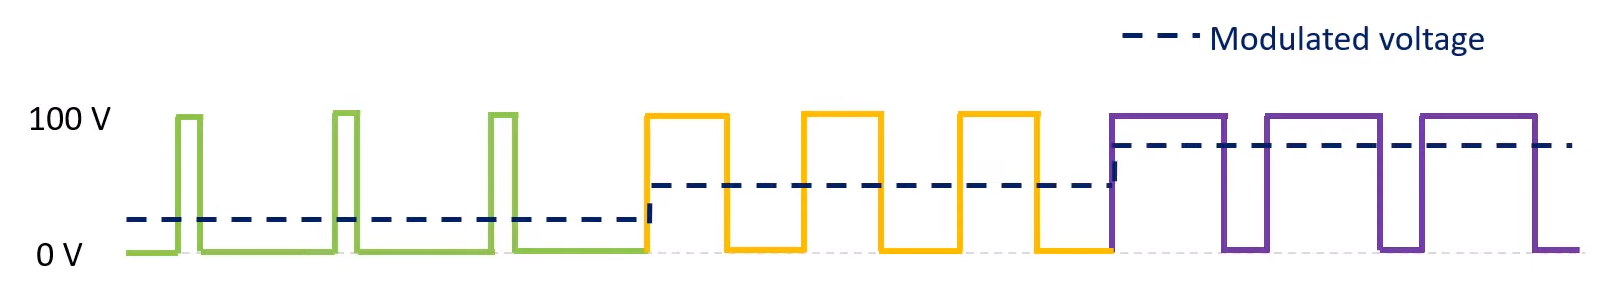
\includegraphics[width=13cm]{imagens/PWM.png}
	\caption*{Fonte:\cite{matlabBLDC}.}
 \label{Modulação por largura de pulso utilizando uma fonte de 100V}
\end{figure}

\subsubsection{Outros Algoritmos de Controle}

Além do Controle Trapezoidal existem outras formas de controle que envolvem algorítimos mais complexos, como o Controle de Torque Vetorial e o Controle de Campo Orientado, ambos em malha fechada.

No controle de torque vetorial, o controlador de motor calcula a corrente que deve ser fornecida às bobinas do estator usando um modelo matemático do motor. O modelo matemático do motor descreve a relação entre a corrente nas bobinas do estator, o campo magnético do rotor e o torque produzido pelo motor. O controlador vetorial de torque do motor calcula o torque desejado e, em seguida, usa o modelo matemático do motor para calcular a corrente necessária para produzir o tal torque. Este controle é um método preciso e flexível que pode ser usado em uma variedade de aplicações. Ele é adequado para aplicações onde a exatidão de velocidade e torque é crítica

No controle de campo orientado, o controlador do motor calcula a corrente que deve ser fornecida às bobinas do estator usando a orientação do campo magnético do rotor. O controlador de motor usa um sensor para medir a orientação do campo magnético do rotor, sendo que o sensor envia um sinal para o controlador, o utiliza sinal para calcular a corrente necessária para manter o campo magnético do rotor na orientação desejada. O controle de campo orientado é um método preciso e eficiente que pode ser usado em aplicações de alta velocidade.

\pagebreak

\subsection{Vantagens e Desvantagens no uso de motores BLDC}
Os motores sem escovas, ou BLDC, apresentam diversas vantagens que contribuem para seu destaque em várias aplicações. O rendimento é uma característica proeminente, uma vez que convertem mais eficientemente a energia elétrica em torque quando comparados aos motores com escovas. Isso implica em uma demanda menor de energia para gerar a mesma quantidade de torque, resultando em um melhor desempenho global. A durabilidade é significativamente aprimorada, visto que a vida útil estendida desses motores está relacionada à ausência das escovas, componentes propensos a desgaste em motores convencionais.

Os motores de indução trifásicos (MIT) são concorrentes diretos dos motores BLDC, sendo que ambos são amplamente utilizados em diversas aplicações, cada uma com suas características distintas e vantagens específicas. Os motores de indução trifásicos são conhecidos pela sua confiabilidade, simplicidade de construção e custo relativamente baixo, quando comparado aos BLDC, utilizando os princípios da indução eletromagnética para gerar o torque e velocidade necessários para a aplicação. Embora tenham menor custo de produção quando comparados com os motores BLDC e podem ser controlados utilizando os mesmos protocolos, os MITs tendem a ter uma densidade de potência e torque menor em comparação com os motores BLDC, principalmente em baixas velocidades, o que pode ser uma consideração importante em aplicações que requerem alta potência em um espaço limitado. No entanto, os MITs apresentam melhor rendimento em operações de baixo torque, o que pode ser relevante em aplicações de mobilidade, como em veículos elétricos.

Os motores BLDC são conhecidos por seu rendimento energético superior, controle preciso de velocidade e torque, além de uma vida útil mais longa devido à ausência de escovas mecânicas \cite{gieras2009permanent}. Embora os BLDCs tenham um custo inicial mais elevado em comparação com os MITs, eles oferecem uma operação mais eficiente, especialmente em condições de carga variável e velocidade ajustável.

Em resumo, os motores sem escovas oferecem um conjunto de vantagens notáveis, incluindo rendimento aprimorado, operação mais silenciosa, maior durabilidade e menor necessidade de manutenção. Contudo, esses benefícios vêm com um custo inicial mais elevado e a exigência de um controlador de velocidade, o que pode tornar sua implementação menos acessível em certos contextos. A escolha entre motores com escovas e sem escovas dependerá das prioridades específicas de uma aplicação, considerando tanto os benefícios quanto as limitações de cada tecnologia.

\pagebreak

\subsection{Aplicações}
Os motores BLDC são amplamente utilizados em diversas aplicações devido às suas características únicas, como elevado rendimento, alta densidade de potência, baixo ruído, baixa manutenção e longa vida útil. Esses motores são preferidos em aplicações que necessitam de controle preciso de torque com oscilações inferiores em comparação com outros motores.

Uma das principais aplicações dos motores BLDC é em veículos elétricos, como carros, motocicletas, bicicletas e \textit{scooters} \cite{chau2007emerging}. Com o aumento da demanda por veículos elétricos, espera-se que os motores com tecnologia derivada do BLDC desempenhem um papel vital na indústria automotiva. Esses motores são usados para acionar o sistema de propulsão do veículo, fornecendo torque e potência para as rodas. Eles são preferidos em veículos elétricos devido à seu alta rendimento, baixo ruído e baixa manutenção. Essas motores são usados em aplicações que exigem alta precisão, controle de velocidade e torque, e baixo ruído.

\section{Objetivos}
Estudar o princípio de funcionamento de um controlador de motores Brushless, tornando possível o projeto e desenvolvimento de um protótipo que possa oferecer uma operação suave e precisa em diferentes cenários de aplicação.

\section{Metodologia}
O desenvolvimento do ESC será realizado em três etapas principais. A primeira conta com uma simulação computacional do sistema para entender a transformação da energia elétrica e a coordenação dos chaveamentos, analisando o controle de rotação e velocidade do motor. Em seguida, na fase de projeto, serão definidos os requisitos mínimos, escolhidos os componentes eletrônicos e desenvolvido o circuito, incluindo controle de tensão, corrente com sinais PWM e proteções. Por último, na prototipagem, o controlador será montado em uma PCB, programado e testado em laboratório para garantir o funcionamento e identificar melhorias.

\subsection{Simulação}
Para o desenvolvimento de um ESC, primeiramente, apresenta-se a simulação do sistema via software, permitindo assim um maior entendimento de cada etapa de transformação da energia elétrica, como a metodologia adotada para coordenação dos chaveamentos, sem as limitações físicas impostas na implementação do circuito real. A simulação gera uma análise teórica funcional sobre o controle de sentido de rotação e velocidade imposta ao motor.

\pagebreak

\subsection{Projeto}
Para a elaboração do projeto físico é necessário o levantamento dos requisitos mínimos que o projeto deve atender, como a categoria de motores que deve atender e sua fonte de alimentação. Em seguida será necessária a seleção dos componentes eletrônicos (drivers, transistores, bateria, entre outros), considerando características como um controlador adequado, tensão de operação, frequência de comutação, corrente máxima suportada e possíveis proteções para o sistema.

O projeto do circuito começa pelo controle de tensão, em seguida será projetado o controle de corrente fornecida às bobinas do motor através de sinais de PWM para controle de velocidade e sentido de rotação, ou seja o drive para motor BLDC e recursos adicionais como proteções térmicas ou de sobrecarga.

\subsection{Prototipagem}
Com o fim do projeto do circuito inicia-se a implementação do controlador em uma placa de circuito impresso (PCB) por meio de um software de design eletrônico. Com a montagem dos componentes na PCB, será necessária a programação do microcontrolador implementado a lógica de chaveamento e outras funções. Também serão realizados teste de funcionamento em laboratório para garantir o funcionamento correto do circuito e levantar possíveis melhorias ou correções. Após as devidas correções serão realizados testes de desempenho afim de verificar se o projeto atende os requisitos estabelecidos de potência e tempo de resposta.

Todas as partes relevantes durante o trabalho de graduação serão documentadas através da redação do relatório acadêmico e apresentação para a defesa do trabalho de graduação.

\section{Cronograma}

O desenvolvimento deste trabalho, está previsto nas seguintes etapas e distribuído de acordo com a Tabela \ref{Cronograma proposto de atividades.}:

\begin{table}[h]
\centering
\caption{Cronograma proposto de atividades.}
\label{Cronograma proposto de atividades.}
\resizebox{\linewidth}{!}{%
\begin{tabular}{|c|l|c|c|c|c|c|c|c|c|c|l|} 
\cline{3-12}
\multicolumn{1}{c}{} & \multicolumn{1}{c|}{} & \multicolumn{10}{c|}{\textbf{Mês}} \\ 
\cline{3-12}
\multicolumn{1}{l}{} &  & \multicolumn{5}{c|}{2024} & \multicolumn{5}{c|}{2025} \\ 
\cline{3-12}
\multicolumn{1}{c}{} & \multicolumn{1}{c|}{} & 08 & 09 & 10 & 11 & 12 & 01 & 02 & 03 & 04 & 05 \\ 
\hline
\multirow{7}{*}{\textbf{Atividades}} & Simulação & {\cellcolor[rgb]{0.753,0.753,0.753}} & {\cellcolor[rgb]{0.753,0.753,0.753}} &  &  &  &  &  &  &  &  \\ 
\hhline{|~-----------|}
 & Projeto do Circuito &  &  & {\cellcolor[rgb]{0.753,0.753,0.753}} & {\cellcolor[rgb]{0.753,0.753,0.753}} & {\cellcolor[rgb]{0.753,0.753,0.753}} &  &  &  &  &  \\ 
\hhline{|~-----------|}
 & Protipagem &  &  &  &  &  & {\cellcolor[rgb]{0.753,0.753,0.753}} &  &  &  &  \\ 
\hhline{|~-----------|}
 & Testes &  &  &  &  &  &  & {\cellcolor[rgb]{0.753,0.753,0.753}} &  &  &  \\ 
\hhline{|~-----------|}
 & Correções e Melhorias &  &  &  &  &  &  &  & {\cellcolor[rgb]{0.753,0.753,0.753}} &  &  \\ 
\hhline{|~-----------|}
 & Testes de Desempenho &  &  &  &  &  &  &  &  & {\cellcolor[rgb]{0.753,0.753,0.753}} &  \\ 
\hhline{|~-----------|}
 & Conclusão &  &  &  &  &  &  &  &  &  & {\cellcolor[rgb]{0.753,0.753,0.753}} \\
\hline
\end{tabular}
}
\caption*{Fonte:Produção do próprio autor.}
\end{table}

%% Bibliografia
\newpage
\printbibliography[heading=bibintoc, title={Bibliografia}]
\pagebreak

%% Assinaturas
\newpage
\section*{Assinaturas}
\addcontentsline{toc}{section}{Assinaturas}

\begin{center}

\vspace{2cm}
\begin{tabular}{@{}p{7cm}@{}}
	\hrulefill       \\

	\textbf{Aluno:} \\
	Enzo Luiz Fernandes
\end{tabular}


\vspace{2cm}
\begin{tabular}{@{}p{7cm}@{}}
	\hrulefill                     \\
	\textbf{Professor Orientador:} \\
	Guilherme de Azevedo Melo
\end{tabular}

\end{center}
\pagebreak

%-----------------------------------------------
\end{document}